% !TeX root=../main.tex

\chapter{روش پیشنهادی}
\label{ch:method}

\section{مقدمه}
این فصل، پیاده‌سازی دقیق ایده‌ای را شرح می‌دهد که در فصل اول معرفی شد: ریزتنظیم یک مدل زبانی، به‌گونه‌ای که بازنمایی جفت‌جمله‌های هم‌معنی و ناهم‌معنی مجموعه‌دادهٔ
\lr{PAWS}
در فضای نهان یک خودرمزگذار پراکندهٔ ثابت، بهتر از یکدیگر تفکیک شوند. ساختار فصل به این ترتیب است: ابتدا نمای کلی معماری و جریان داده در بخش~\ref{sec:overview} ارائه می‌شود؛ سپس مدل پایه و روش تطبیق کارآمد پارامتر (بخش~\ref{sec:base-model})، دادگان (بخش~\ref{sec:data})، و مکانیسم خودرمزگذار ثابت و قلاب‌کردن جریان باقیمانده (بخش~\ref{sec:sae}) معرفی می‌شوند. بخش~\ref{sec:loss} تابع هزینهٔ کامل را با جزئیات ریاضی شرح می‌دهد، بخش~\ref{sec:conditions} چهار شرط آزمایشی را تعریف می‌کند، بخش~\ref{sec:ablation} طرح آزمایش‌های شبکه‌ای را می‌آورد، بخش~\ref{sec:metrics} معیارهای ارزیابی را تعریف می‌کند و سرانجام بخش~\ref{sec:impl} جزئیات پیاده‌سازی و ابرپارامترها را فهرست می‌کند.

\section{نمای کلی معماری}
\label{sec:overview}
شکل~\ref{fig:architecture} جریان کلی داده و محاسبهٔ تابع هزینه را نشان می‌دهد. در هر گام از آموزش، دو دستهٔ داده به‌طور موازی از یک مدل مشترک (مدل پایه به‌همراه تطبیق‌دهندهٔ لورا؛ بخش~\ref{sec:base-model}) عبور داده می‌شوند و در نهایت، چهار جزء تابع هزینه را می‌سازند که مجموعشان، تابع هزینهٔ نهایی است.

\paragraph{مسیر \lr{PAWS} (نیمهٔ بالایی شکل).}
یک دستهٔ جفت‌جمله--شامل چند جفت هم‌معنی و چند جفت ناهم‌معنی--از مدل عبور داده می‌شود. فعال‌سازی هر جمله در لایهٔ هدف قلاب و گرفته می‌شود، و پس از عبور از خودرمزگذار ثابت (رمزگذاری)، به کدی نهان تبدیل می‌شود. از این نقطه، دو مسیر موازی طی می‌شود: در مسیر نخست، کدهای نهان هر جمله تجمیع (میانگین‌گیری روی نشانه‌ها) شده و شباهت کسینوسی آن‌ها، مبنای تابع هزینهٔ ناوردایی قرار می‌گیرد؛ در مسیر دوم--که مستقل از تجمیع است--همان کدهای نهان از خودرمزگذار رمزگشایی می‌شوند و خطای بازسازی حاصل، مبنای منظم‌ساز بازسازی روی دستهٔ
\lr{PAWS}
قرار می‌گیرد.

\paragraph{مسیر \lr{WikiText} (نیمهٔ پایین شکل).}
یک دستهٔ متن عمومی از پیکرهٔ
\lr{WikiText-2}
نیز از همان مدل عبور داده می‌شود و به دو منظور به کار می‌رود: نخست، محاسبهٔ هزینهٔ آنتروپی متقاطع استاندارد زبان‌مدل‌سازی؛ دوم، قلاب‌کردن فعال‌سازی همین دسته در لایهٔ هدف و عبور آن از خودرمزگذار ثابت (رمزگذاری و سپس بلافاصله رمزگشایی) برای محاسبهٔ منظم‌ساز بازسازی روی دستهٔ
\lr{WikiText}.

\paragraph{همگرایی در تابع هزینهٔ کل.}
هر چهار جزء--هزینهٔ زبان‌مدل‌سازی، منظم‌ساز بازسازی
\lr{WikiText}، تابع هزینهٔ ناوردایی، و منظم‌ساز بازسازی
\lr{PAWS}--در تابع هزینهٔ نهایی جمع می‌شوند (فرمول دقیق در بخش~\ref{sec:loss}). تنها گرادیان همین تابع هزینهٔ نهایی است که به پارامترهای قابل‌آموزش--یعنی تطبیق‌دهندهٔ لورا، به‌علاوهٔ دو پارامتر مقیاس و بایاس تابع هزینهٔ ناوردایی--بازمی‌گردد؛ همان‌طور که در شکل با حاشیهٔ نقطه‌چین مشخص شده، پارامترهای خود خودرمزگذار در هر دو مسیر، در سرتاسر آموزش کاملاً ثابت می‌مانند و هیچ گرادیانی به داخل آن‌ها انباشته نمی‌شود.

\begin{figure}[htb]
\centering
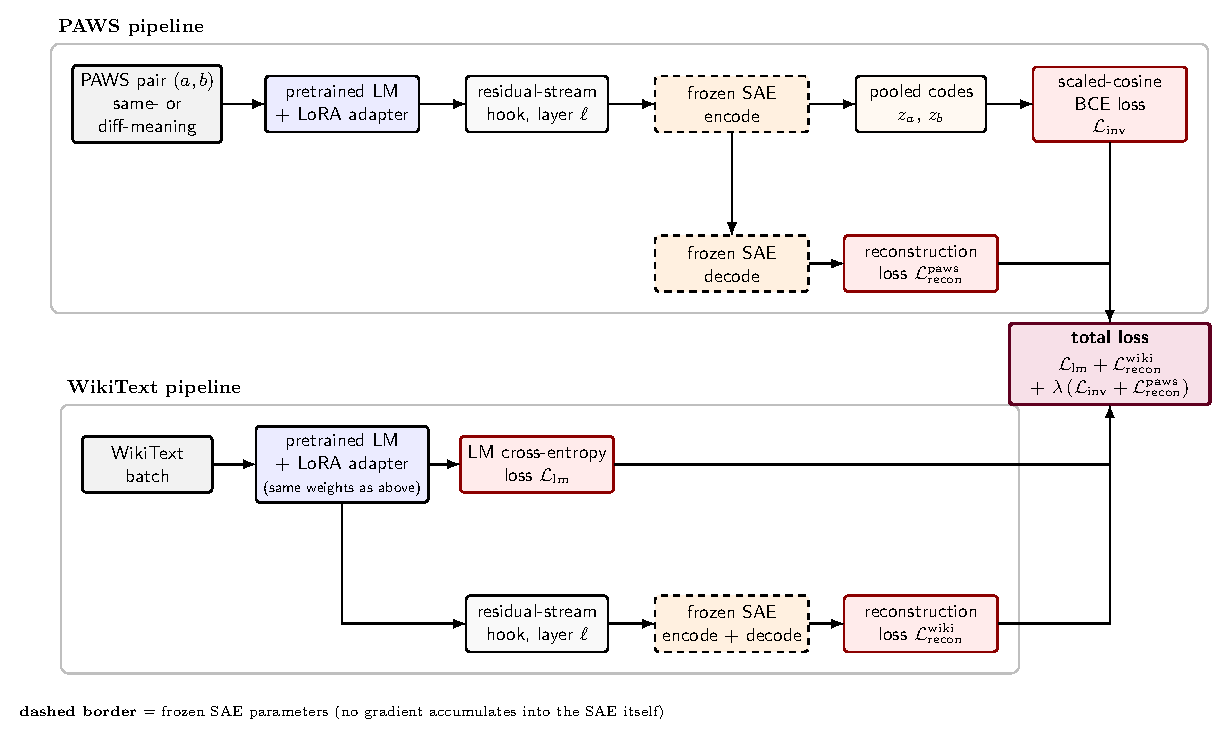
\includegraphics[width=\textwidth]{architecture_diagram}
\caption{نمای کلی معماری و جریان محاسبهٔ تابع هزینه. پنل بالا مسیر جفت‌جمله‌های \lr{PAWS} را نشان می‌دهد که هم به تابع هزینهٔ ناوردایی و هم به منظم‌ساز بازسازی خود \lr{PAWS} می‌انجامد؛ پنل پایین مسیر \lr{WikiText} را نشان می‌دهد که هم به هزینهٔ زبان‌مدل‌سازی و هم به منظم‌ساز بازسازی \lr{WikiText} می‌انجامد. کادرهای با حاشیهٔ نقطه‌چین (خودرمزگذار ثابت) پارامترهایی را نشان می‌دهند که هرگز به‌روزرسانی نمی‌شوند؛ گرادیان تنها از طریق تطبیق‌دهندهٔ لورای مشترک (که در هر دو پنل، همان وزن‌های یکسان است) به پارامترهای قابل‌آموزش بازمی‌گردد.}
\label{fig:architecture}
\end{figure}

\section{مدل پایه و تطبیق کارآمد پارامتر}
\label{sec:base-model}
مدل پایهٔ مورد استفاده در تمام آزمایش‌های این پایان‌نامه،
\lr{Pythia-70m-deduped}~\cite{biderman2023pythia}
است: عضو کوچک‌ترین خانوادهٔ مدل‌های
\lr{Pythia}، توسعه‌یافته توسط
\lr{EleutherAI}
بر پایهٔ معماری
\lr{GPT-NeoX}~\cite{black2022gptneox}
و پیش‌آموزش‌دیده روی نسخهٔ حذف‌تکرارشدهٔ\LTRfootnote{Deduplicated}
پیکرهٔ
\lr{The Pile}~\cite{gao2020pile}. این مدل ۶ لایهٔ ترنسفورمر و ابعاد جریان باقیماندهٔ ۵۱۲ دارد. انتخاب این مدل، دو دلیل عملی داشت: نخست، خانوادهٔ
\lr{Pythia}
به‌طور خاص برای پژوهش‌های تحلیلی و قابلیت تکرارپذیری طراحی شده است~\cite{biderman2023pythia}؛ دوم، وجود مجموعه‌ای از خودرمزگذارهای پراکندهٔ از پیش‌آموزش‌دیده و عمومی برای این مدل (قابل‌بارگذاری از طریق کتابخانهٔ
\lr{SAELens}~\cite{bloom2024saelens})، پیش‌نیاز مستقیم روش پیشنهادی را برآورده می‌کند. کوچکی این مدل همچنین امکان اجرای شبکهٔ آزمایشی نسبتاً بزرگ این پژوهش (بخش~\ref{sec:ablation}) را در محدودهٔ منابع محاسباتی در دسترس فراهم کرد؛ در فصل پنجم به این انتخاب و پیامدهای آن برای تعمیم‌پذیری نتایج بازمی‌گردیم.

برای ریزتنظیم کارآمد پارامتر، از روش
لورا\LTRfootnote{Low-Rank Adaptation, LoRA}~\cite{hu2021lora}
استفاده شده است. لورا به‌جای به‌روزرسانی مستقیم ماتریس‌های وزن از پیش‌آموزش‌دیده، برای هر ماتریس هدف
$W_0 \in \mathbb{R}^{d \times k}$
یک به‌روزرسانی کم‌رتبه به شکل
$\Delta W = BA$
می‌افزاید، که در آن
$B \in \mathbb{R}^{d \times r}$
و
$A \in \mathbb{R}^{r \times k}$
با
$r \ll \min(d,k)$
هستند و تنها همین دو ماتریس کوچک آموزش داده می‌شوند؛ خروجی لایه به‌صورت
$W_0 x + \frac{\alpha}{r}BAx$
محاسبه می‌شود، که در آن
$\alpha$
یک ضریب مقیاس‌دهی ثابت است. در این پژوهش، لورا روی ماتریس‌های تصویر ترکیبی پرسمان--کلید--مقدار و تصویر خروجی بلوک توجه اعمال شده است؛ مقادیر دقیق رتبه، ضریب مقیاس، و دراپ‌اوت در پیوست «الف» فهرست شده‌اند. تمام لایه‌های مدل به‌طور یکسان تطبیق‌پذیرند؛ آنچه میان شرایط مختلف آزمایشی تغییر می‌کند، محل اعمال تابع هزینهٔ ناوردایی است (بخش~\ref{sec:ablation})، نه محل اعمال لورا.

\section{دادگان}
\label{sec:data}
دو منبع داده در آموزش نقش دارند:

\paragraph{\lr{PAWS}.}
مجموعه‌دادهٔ
\lr{PAWS}~\cite{zhang2019paws}
(زیرمجموعهٔ
\lr{labeled\_final})
منبع سیگنال نظارتی اصلی است. هر جفت‌جمله برچسب دودویی هم‌معنی/ناهم‌معنی دارد. برای هر یک از سه شکاف استاندارد (آموزش، اعتبارسنجی، آزمون)، به‌طور مستقل، تعداد برابری جفت هم‌معنی و ناهم‌معنی--با یک بذر تصادفی ثابت برای تکرارپذیری--نمونه‌برداری شده است؛ اندازهٔ دقیق هر شکاف در پیوست «الف» آمده است. شکاف آزمون، تا پایان آموزش هر پیکربندی، هرگز مورد استفاده قرار نمی‌گیرد و تنها در مرحلهٔ ارزیابی نهایی (فصل چهارم) به کار می‌رود؛ شکاف اعتبارسنجی، برای پایش دوره‌ای سلامت آموزش (بخش~\ref{sec:impl}) استفاده می‌شود.

\paragraph{\lr{WikiText-2}.}
برای جلوگیری از افت کیفیت عمومی زبان‌مدل‌سازی در حین ریزتنظیم متمرکز بر
\lr{PAWS}
(پدیده‌ای که در ادبیات یادگیری پیوسته با عنوان فراموشی فاجعه‌بار\LTRfootnote{Catastrophic Forgetting}
شناخته می‌شود~\cite{kirkpatrick2017ewc})، در هر گام آموزش، یک دستهٔ متن عمومی نیز از نسخهٔ خام
\lr{WikiText-2}
نمونه‌برداری و همراه با دستهٔ
\lr{PAWS}
از مدل عبور داده می‌شود. متن خام به بلوک‌هایی با طول ثابت بریده می‌شود؛ بخش پایانی مجموعه برای اعتبارسنجی کنار گذاشته شده و باقی برای آموزش استفاده می‌شود.

\section{خودرمزگذار پراکندهٔ ثابت}
\label{sec:sae}
برای هر لایهٔ مدل، یک خودرمزگذار پراکنده\LTRfootnote{Sparse Autoencoder, SAE}
از پیش‌آموزش‌دیده و عمومی (منتشرشده در مخزن
\lr{SAELens}~\cite{bloom2024saelens}) بارگذاری می‌شود. این خودرمزگذار، بردار فعال‌سازی جریان باقیمانده را (پس از هر بلوک، یعنی در نقطهٔ قلاب استاندارد
\lr{hook\_resid\_post}) به یک کد پراکنده با ابعاد بسیار بیشتر می‌برد، و سپس تلاش می‌کند از روی همین کد، بردار اصلی را بازسازی کند. تابع رمزگذاری و رمزگشایی آن را به‌ترتیب با
$\mathrm{Enc}(\cdot)$
و
$\mathrm{Dec}(\cdot)$
نشان می‌دهیم.

نکتهٔ کلیدی پیاده‌سازی آن است که تمام پارامترهای این خودرمزگذار، در سرتاسر آموزش، منجمد نگه داشته می‌شوند: هیچ گرادیانی \emph{به داخل} پارامترهای خودرمزگذار انباشته نمی‌شود. با این‌همه، از آنجا که منجمدبودن یک ماژول مانع عبور گرادیان \emph{از میان} آن به ورودی‌اش نمی‌شود، سیگنال گرادیانی حاصل از تابع هزینه‌ای که روی خروجی
$\mathrm{Enc}(\cdot)$
محاسبه شده، همچنان می‌تواند از میان خودرمزگذار عبور کرده و به فعال‌سازی‌های مدل--و از آن‌جا، به پارامترهای لورا--برسد. همین ویژگی است که امکان استفاده از خودرمزگذار به‌عنوان «عدسی ثابت» تابع هزینه (نه هدف آموزش) را فراهم می‌کند؛ الگویی مشابه با استفاده از یک شبکهٔ ثابت از پیش‌آموزش‌دیده در تابع هزینه‌های ادراکی\LTRfootnote{Perceptual Loss}
در بینایی ماشین.

\subsection{ریسک رانش خودرمزگذار و راه‌حل پیشنهادی}
\label{sec:sae-drift}
استفاده از یک خودرمزگذار ثابت به‌عنوان ابزار سنجش، به این فرض متکی است که فعال‌سازی‌های مدل، پس از ریزتنظیم، همچنان در ناحیه‌ای از فضای فعال‌سازی قرار داشته باشند که این خودرمزگذار روی آن آموزش دیده و می‌تواند آن را با دقت قابل‌قبولی بازسازی کند. اگر ریزتنظیم فعال‌سازی‌ها را به‌گونه‌ای جابه‌جا کند که این فرض نقض شود--پدیده‌ای که در این پایان‌نامه «رانش خودرمزگذار»\LTRfootnote{SAE Drift}
نامیده می‌شود--آنگاه هر سنجه‌ای که در فضای این خودرمزگذار محاسبه شود (از جمله سنجهٔ اصلی این پژوهش، یعنی جدایی هم‌معنی/ناهم‌معنی در فضای
\lr{SAE}) دیگر لزوماً بازتابی از تغییر واقعی در بازنمایی مدل نیست، بلکه می‌تواند بازتابی از عبور فعال‌سازی‌ها از میان یک ابزار سنجش نامنطبق باشد.

برای مهار این ریسک، خودرمزگذار در سرتاسر آموزش کاملاً ثابت نگه داشته می‌شود (بدون هیچ تغییری در وزن‌های خودش)، و در عوض، هزینهٔ بازسازی آن--محاسبه‌شده هم روی فعال‌سازی‌های دستهٔ
\lr{WikiText}
و هم روی فعال‌سازی‌های دستهٔ
\lr{PAWS}--به‌عنوان یک جزء اضافی به تابع هزینهٔ کلی افزوده می‌شود. از آنجا که خودرمزگذار ثابت است، تنها مسیری که این جزء گرادیان می‌تواند طی کند، بازگشت از میان خودرمزگذار به خود فعال‌سازی‌ها--یعنی به پارامترهای لورایی است که این فعال‌سازی‌ها را تولید کرده‌اند. نتیجه، نیرویی است که مدل را وامی‌دارد در ناحیه‌ای از فضای فعال‌سازی بماند که خودرمزگذار همچنان می‌تواند آن را با وفاداری قابل‌قبولی بازسازی کند؛ این سازوکار از نظر مفهومی با جریمهٔ واگرایی کولبک--لایبلر نسبت به یک سیاست مرجع در یادگیری تقویتی مبتنی بر بازخورد انسانی~\cite{ouyang2022instructgpt} قابل‌مقایسه است: در هر دو مورد، یک جزء تابع هزینه، مدل را از دورشدن بیش‌ازحد از یک نقطهٔ مرجع ثابت (به‌ترتیب، خودرمزگذار از پیش‌آموزش‌دیده، یا سیاست پیش‌آموزش‌دیده) بازمی‌دارد، درحالی‌که جزء دیگر تابع هزینه مدل را در جهت هدف اصلی (به‌ترتیب، جداسازی هم‌معنی/ناهم‌معنی، یا هم‌سویی رفتاری) پیش می‌برد. تمام نتایج این پایان‌نامه با همین رویکرد--خودرمزگذار کاملاً ثابت به‌همراه منظم‌ساز بازسازی--به دست آمده‌اند.

\subsection{فرمول منظم‌ساز بازسازی}
با فرض آنکه
$X$
دسته‌ای از بردارهای فعال‌سازی باشد، خطای بازسازی نرمال‌شدهٔ این دسته به‌صورت نسبت \emph{مجموع} خطاهای مربعی به \emph{مجموع} نُرم‌های مربعی تعریف می‌شود:
\begin{equation}
\label{eq:recon}
\mathcal{L}_{\mathrm{recon}}(X) = \frac{\sum_{x \in X} \lVert \mathrm{Dec}(\mathrm{Enc}(x)) - x \rVert_2^2}{\sum_{x \in X} \lVert x \rVert_2^2}
\end{equation}
نکتهٔ فنی مهم در این فرمول، جمع‌بندی‌کردن صورت و مخرج \emph{پیش از} تقسیم است، نه میانگین‌گیری از نسبت‌های تک‌تک نشانه‌ها. این انتخاب، پاسخ به یک اشکال ناپایداری واقعی است که در مراحل اولیهٔ توسعهٔ این پروژه مشاهده شد: با فرمول میانگین نسبت‌ها، وجود حتی یک نشانه با نُرم فعال‌سازی نزدیک به صفر در یک دسته می‌توانست جملهٔ به‌شدت بزرگ و نامتناسبی در میانگین تولید کند و برای یک گام، کل آموزش را ناپایدار سازد؛ فرمول تجمیعی رابطهٔ~\ref{eq:recon}، در برابر چنین دورافتاده‌هایی مقاوم است، چون سهم یک نشانهٔ منفرد در مجموع مخرج (نه در یک تقسیم مجزا) گم می‌شود. در پیاده‌سازی عملی، برای پایداری عددی بیشتر، یک ثابت کوچک به مخرج افزوده و خروجی نهایی از بالا کران‌دار می‌شود؛ مقادیر دقیق این دو ثابت در پیوست «الف» فهرست شده‌اند.

سنجهٔ مکملی که در فصل چهارم برای پایش این خطا در طول آموزش گزارش می‌شود، \emph{واریانس تبیین‌شدهٔ بازسازی} است و به‌سادگی برابر با
$1-\mathcal{L}_{\mathrm{recon}}$
تعریف می‌شود.

\section{تابع هزینه}
\label{sec:loss}
تابع هزینهٔ کلی هر گام آموزشی، مجموع چهار جزئی است که در بخش~\ref{sec:overview} معرفی شدند:
\begin{equation}
\label{eq:total}
\mathcal{L}_{\mathrm{total}} = \mathcal{L}_{\mathrm{lm}} + \mathcal{L}_{\mathrm{recon}}^{\mathrm{wiki}} + \lambda \left( \mathcal{L}_{\mathrm{inv}} + \mathcal{L}_{\mathrm{recon}}^{\mathrm{paws}} \right)
\end{equation}
که در آن
$\mathcal{L}_{\mathrm{lm}}$
هزینهٔ آنتروپی متقاطع استاندارد زبان‌مدل‌سازی روی دستهٔ
\lr{WikiText}
است،
$\mathcal{L}_{\mathrm{recon}}^{\mathrm{wiki}}$
منظم‌ساز بازسازی رابطهٔ~\ref{eq:recon} محاسبه‌شده روی فعال‌سازی‌های همان دستهٔ
\lr{WikiText}
در لایه(های) هدف است،
$\mathcal{L}_{\mathrm{inv}}$
تابع هزینهٔ ناوردایی روی دستهٔ
\lr{PAWS}
است، و
$\mathcal{L}_{\mathrm{recon}}^{\mathrm{paws}}$
همان منظم‌ساز بازسازی است، این‌بار محاسبه‌شده روی فعال‌سازی‌های دستهٔ
\lr{PAWS}. نکتهٔ قابل‌توجه در این فرمول، عدم‌تقارن وزن‌دهی است: ضریب
$\lambda$
تنها روی جزء متمرکز بر
\lr{PAWS}
(هم تابع هزینهٔ ناوردایی و هم منظم‌ساز بازسازی متناظر با آن) اعمال می‌شود، درحالی‌که مسیر متمرکز بر
\lr{WikiText}
همواره با وزن ثابت یک در تابع هزینه حاضر است. پیامد این عدم‌تقارن آن است که با افزایش
$\lambda$، وزن نسبی مسیر نگه‌دارندهٔ سلامت عمومی (زبان‌مدل‌سازی و بازسازی
\lr{WikiText}) در برابر مسیر متمرکز بر
\lr{PAWS}
کاهش می‌یابد؛ در فصل چهارم (بخش~\ref{sec:res-dynamics}) نشان داده می‌شود این عدم‌تقارن، تبیین محتملی برای هزینهٔ پایداری‌ای است که در وزن‌های بالای
$\lambda$
مشاهده می‌شود.

\subsection{تابع هزینهٔ ناوردایی}
برای محاسبهٔ
$\mathcal{L}_{\mathrm{inv}}$، ابتدا از هر جمله در دستهٔ
\lr{PAWS}
یک بردار تکی ساخته می‌شود: فعال‌سازی هر نشانهٔ آن جمله در لایهٔ هدف گرفته می‌شود و--بسته به شرط آزمایشی--یا مستقیماً میانگین‌گیری می‌شود (فضای خام)، یا نخست از میان
$\mathrm{Enc}(\cdot)$
عبور داده شده و سپس میانگین‌گیری می‌شود (فضای
\lr{SAE}؛ یعنی رمزگذاری پیش از تجمیع، نه برعکس، تا ورودی خودرمزگذار همواره در توزیعی بماند که برای آن آموزش دیده است). برای یک دستهٔ
$B$
جفت هم‌معنی
$\{(a_i, b_i)\}_{i=1}^{B}$
و
$B$
جفت ناهم‌معنی
$\{(a'_i, b'_i)\}_{i=1}^{B}$، شباهت کسینوسی هر جفت محاسبه می‌شود:
$s_i^{\mathrm{same}} = \cos(z_{a_i}, z_{b_i})$
و
$s_i^{\mathrm{diff}} = \cos(z_{a'_i}, z_{b'_i})$، که در آن
$z$
بردار تجمیع‌شده (خام یا
\lr{SAE}) است.

این
$2B$
مقدار شباهت، با یک مقیاس آموختنی
$\gamma$
و یک بایاس آموختنی
$\beta$
به لوجیت تبدیل و با تابع هزینهٔ آنتروپی متقاطع دودویی زیر ترکیب می‌شوند:
\begin{equation}
\mathcal{L}_{\mathrm{bce}} = -\frac{1}{2B}\left[
\sum_{i=1}^{B} \log \sigma(\gamma s_i^{\mathrm{same}} + \beta)
+ \sum_{i=1}^{B} \log\big(1 - \sigma(\gamma s_i^{\mathrm{diff}} + \beta)\big)
\right]
\end{equation}
با
$\sigma$
تابع سیگموید. این صورت‌بندی--که این پایان‌نامه از آن با نام «\lr{BCE} کسینوسی مقیاس‌پذیر» یاد می‌کند--جایگزین یک تابع هزینهٔ hinge با حاشیهٔ ثابت است: به‌جای تعریف دستی یک آستانهٔ جداکنندهٔ ثابت میان جفت‌های هم‌معنی و ناهم‌معنی، مقیاس و بایاس در حین آموزش یاد گرفته می‌شوند و مرز جداکننده را خودشان تطبیق می‌دهند. در پیاده‌سازی عملی، مقیاس
$\gamma$
از بالا کران‌دار می‌شود تا از یک راه میان‌بُر بی‌ربط به هدف اصلی جلوگیری شود: بدون این کران، مدل می‌تواند به‌جای دورترکردن واقعی بازنمایی‌ها، صرفاً
$\gamma$
را به‌طور نامحدود بزرگ کند تا شیب سیگموید حول هر جدایی موجود--هرچند ناچیز--تیزتر و در نتیجه، تابع هزینه کوچک‌تر شود؛ مقدار دقیق این کران در پیوست «الف» آمده است.

برای شرط
\lr{C4} (بخش~\ref{sec:conditions})، یک جزء مکمل اختیاری نیز--تنها برای جفت‌های هم‌معنی و تنها در فضای
\lr{SAE}--افزوده می‌شود: تقریب نرم و مشتق‌پذیر فاصلهٔ همپوشانی تکیه‌گاه\LTRfootnote{Support Overlap}
(نسخهٔ نرم‌شدهٔ سنجهٔ دایس\LTRfootnote{Dice}):
\begin{equation}
\mathcal{L}_{\mathrm{support}} = 1 - \frac{2\sum_j \min(z_{a,j}, z_{b,j})}{\sum_j z_{a,j} + \sum_j z_{b,j}}
\end{equation}
که در آن
$j$
بر روی بُعدهای کد
\lr{SAE}
اندیس می‌زند (کدها به‌دلیل معماری
\lr{ReLU}-پایه، نامنفی هستند). این جزء، برخلاف جزء
\lr{BCE}
که تنها بر \emph{راستای}
بردارها (از طریق شباهت کسینوسی) حساس است، مستقیماً به \emph{هم‌پوشانی مجموعهٔ ویژگی‌های فعال} در دو جمله حساس است: دو کد پراکنده می‌توانند شباهت کسینوسی بالایی داشته باشند درحالی‌که مجموعهٔ ویژگی‌های فعالشان تفاوت محسوسی دارد؛ جزء حمایتی برای سخت‌گیرانه‌ترکردن معیار «هم‌معنی‌بودن» در فضای
\lr{SAE}
افزوده شده است.

\section{شرایط آزمایشی}
\label{sec:conditions}
برای امکان مقایسهٔ علّی--یعنی برای پاسخ‌دادن به این پرسش که آیا اثر مشاهده‌شده واقعاً از \emph{انتخاب فضای}
\lr{SAE}
ناشی می‌شود یا صرفاً از \emph{وجود} هر نوع هدف ناوردایی--چهار شرط آزمایشی تعریف شده‌اند که تنها در یک یا دو مؤلفه با یکدیگر تفاوت دارند. جدول~\ref{tab:conditions} این شرایط را خلاصه می‌کند.

\begin{table}[htb]
\centering
\caption{شرایط آزمایشی. ستون «فضا» فضایی را نشان می‌دهد که تابع هزینهٔ ناوردایی در آن محاسبه می‌شود.}
\label{tab:conditions}
\begin{tabular}{lllll}
\toprule
شرط & توضیح & فضا & \lr{BCE} & جزء حمایتی \\
\midrule
\lr{C1} (کنترل) & بدون تابع هزینهٔ ناوردایی & --- & --- & --- \\
\lr{C2} & ناوردایی در فضای خام & خام & \checkmark & --- \\
\lr{C3} & ناوردایی در فضای \lr{SAE} & \lr{SAE} & \checkmark & --- \\
\lr{C4} & ناوردایی در فضای \lr{SAE} + حمایت & \lr{SAE} & \checkmark & \checkmark \\
\bottomrule
\end{tabular}
\end{table}

شرط
\lr{C1}
به‌عنوان خط پایهٔ کنترلی عمل می‌کند: مدل تنها با هزینهٔ زبان‌مدل‌سازی (و منظم‌ساز بازسازی
\lr{WikiText}) ریزتنظیم می‌شود، بدون آنکه هیچ سیگنالی از
\lr{PAWS}
ببیند. مقایسهٔ
\lr{C1}
با سه شرط دیگر، امکان پاسخ به این پرسش را می‌دهد که آیا صرف ریزتنظیم‌کردن مدل--بدون هیچ هدف مشخصی دربارهٔ جداسازی معنایی--به‌خودی‌خود می‌تواند جداسازی هم‌معنی/ناهم‌معنی را تغییر دهد. مقایسهٔ
\lr{C2}
با
\lr{C3}
مستقیماً فرضیهٔ محوری این پایان‌نامه را می‌آزماید: با ثابت‌نگه‌داشتن همهٔ اجزای دیگر تابع هزینه، تنها تفاوت این دو شرط، فضایی است که در آن شباهت کسینوسی محاسبه می‌شود. مقایسهٔ
\lr{C3}
با
\lr{C4}
نیز اثر جزء حمایتی تکمیلی را، مستقل از جزء اصلی
\lr{BCE}، می‌سنجد.

\section{طرح آزمایش‌های شبکه‌ای}
\label{sec:ablation}
فراتر از چهار شرط بالا، دو ابرپارامتر دیگر نیز به‌طور سیستماتیک تغییر داده شده‌اند:

\paragraph{وزن تابع هزینهٔ ناوردایی ($\lambda$).}
برای هر یک از سه شرط دارای تابع هزینهٔ ناوردایی
(\lr{C2}، \lr{C3}، \lr{C4})، پنج مقدار
$\lambda$
--از بسیار کوچک تا نسبتاً بزرگ--آزموده شده است؛ مقادیر دقیق در پیوست «الف» آمده‌اند. شرط
\lr{C1}
از این ابرپارامتر مستقل است (تنها یک بار اجرا می‌شود).

\paragraph{لایه(های) هدف.}
تابع هزینهٔ ناوردایی و منظم‌ساز بازسازی
\lr{PAWS}
می‌توانند هم‌زمان روی یک یا چند لایه اعمال شوند (در این حالت، رابطهٔ~\ref{eq:total} روی مجموع لایه‌های هدف جمع‌بندی می‌شود). ده حالت متفاوت برای این انتخاب آزموده شده‌اند: شش تک‌لایه (تمام لایه‌های این مدل) و چهار ترکیب چندلایهٔ متوالی از لایه‌های میانی-به-بعد؛ فهرست دقیق در پیوست «الف» آمده است.

مجموع این دو محور آزمایش‌های شبکه‌ای--در هر یک از ده حالت انتخاب لایه، سه شرط در پنج مقدار
$\lambda$
به‌علاوهٔ یک اجرای
\lr{C1}--در مجموع ۱۶۰ اجرای ریزتنظیم مستقل، به‌علاوهٔ یک ارزیابی خط پایه روی مدل پیش‌آموزش‌دیدهٔ بدون ریزتنظیم، تولید می‌کند. جدول کامل این شبکهٔ آزمایشی در پیوست «الف» آمده است.

\section{معیارهای ارزیابی}
\label{sec:metrics}
پس از هر اجرای آموزش، مدل حاصل بر روی شکاف آزمون
\lr{PAWS}
و در \emph{تمام} لایه‌های مدل--نه فقط لایه(های) هدف آموزش--ارزیابی می‌شود. برای هر لایه و هر یک از دو فضا (خام و
\lr{SAE})، معیار اصلی گزارش‌شده،
\lr{AUROC}
(سطح زیر منحنی مشخصهٔ عملکرد گیرنده)~\cite{fawcett2006roc}
است: با در نظرگرفتن فاصلهٔ کسینوسی
$1-\cos(z_a,z_b)$
هر جفت به‌عنوان سنجهٔ تفکیک‌کننده،
\lr{AUROC}
احتمال آن است که یک جفت ناهم‌معنی تصادفی، فاصلهٔ بزرگ‌تری از یک جفت هم‌معنی تصادفی داشته باشد؛ مقدار
۵٫۰
معادل حدس تصادفی و مقدار
۱
معادل تفکیک کامل است. تفاوت
$\Delta_{\mathrm{AUROC}} = \mathrm{AUROC}_{\mathrm{SAE}} - \mathrm{AUROC}_{\mathrm{raw}}$
در هر لایه، به‌طور مجزا نیز گزارش می‌شود تا مشخص شود در کدام لایه، فضای
\lr{SAE}
نسبت به فضای خام، تفکیک‌کنندهٔ بهتری است یا نه.

در کنار
\lr{AUROC}، دو معیار مکمل زیر نیز محاسبه می‌شوند:

\begin{description}
\item[سرگشتگی زبان‌مدل‌سازی\LTRfootnote{Perplexity}:]
سرگشتگی مدل روی شکاف اعتبارسنجی
\lr{WikiText}، در هر نقطهٔ بازرسی، به‌عنوان سنجهٔ سلامت عمومی زبان‌مدل‌سازی پایش می‌شود؛ افزایش محسوس این سنجه نسبت به شرط کنترلی، نشانهٔ آن است که ریزتنظیم، به بهای افت کیفیت زبانی مدل، به هدف ناوردایی رسیده است.
\item[واریانس تبیین‌شدهٔ بازسازی:]
همان کمیت معرفی‌شده در بخش~\ref{sec:sae-drift}، محاسبه‌شده روی مخلوط فعال‌سازی‌های
\lr{PAWS}
و
\lr{WikiText}
در هر نقطهٔ بازرسی؛ این سنجه، معیار اصلی پایش سلامت فرض «خودرمزگذار ثابت همچنان معتبر» است.
\end{description}

\section{جزئیات پیاده‌سازی}
\label{sec:impl}
تمام آزمایش‌ها با کتابخانه‌های
\lr{PyTorch}، \lr{HuggingFace Transformers}
و
\lr{PEFT}
(برای لورا)، و
\lr{SAELens}~\cite{bloom2024saelens}
(برای بارگذاری خودرمزگذارهای از پیش‌آموزش‌دیده، با قلاب‌گذاری در نقاط سازگار با قراردادهای
\lr{TransformerLens}~\cite{nanda2022transformerlens}) پیاده‌سازی شده‌اند. هر پیکربندی (ترکیب شرط،
$\lambda$، و لایهٔ هدف) به‌طور مستقل و از ابتدا، با بهینه‌ساز
\lr{AdamW}
و بریدن نرم گرادیان\LTRfootnote{Gradient Clipping}
روی مجموع پارامترهای قابل‌آموزش اجرا شده است. هر تعدادی گام ثابت، معیارهای بخش~\ref{sec:metrics} روی شکاف اعتبارسنجی محاسبه و ثبت می‌شوند. جدول کامل ابرپارامترها--شامل نرخ یادگیری، تعداد گام‌های آموزش، اندازهٔ دسته‌ها، و مقادیر دقیق ثابت‌های پایداری عددی اشاره‌شده در بخش‌های~\ref{sec:sae} و~\ref{sec:loss}--در پیوست «الف» آمده است.
